% !TeX root = ../main.tex

\subsection{Chromatin Coarse-Graining, chromatin as a polymeric fluid}

In a very interesting chapter, which is summarized in this section, the book "\textit{Giant molecules: here, there, and everywhere}"
\cite{grosbergGiantMoleculesHere2011}
compares the DNA to a chain of beads, and more in general, to a polymeric fluid inside the cell nucleus. It affirms that the random motion of a DNA fiber could be compared to the random Brownian motion of a particle: several small connected segments would move randomly, however maintaining their order and connectivity. Given that the difference between a Brownian motion and a straight movement could be written as follows:

\begin{align*}
    &\text{- For a straight motion } \;\;\;\; R = v(t_2 - t_1) \\ 
    &\text{- For a Brownian particle } \;\;\;\; R = l_{\text{eff}}^{1/2} [v (t_2 - t_1)]^{1/2} 
\end{align*}

Where $R = |\vec{R_1} - \vec{R_2}|$ is the difference between the initial position $\vec{R_1}$ and the final one $\vec{R_2}$, the obtained equation can be rewritten as a square-root displacement in the following way:

$$
    R = l_{\text{eff}}^{1/2} [v (t_2 - t_1)]^{1/2} = \langle(\vec{R_2} - \vec{R_1})^2\rangle^{1/2}
$$

By easily substituing $v (t_2 - t_1)$ with $L$

$$
    R = l_{\text{eff}}^{1/2} * L^{1/2}
$$

Where L is the maximal possible length of the polymer, and is called contour length. By taking the square of the previous equation, it is possible to obtain

\begin{align} \label{eq: kuhn length definition}
    & R^2 = l_{\text{eff}} * L = \langle\vec{R}^2\rangle \nonumber\\ 
    & \rightarrow l_{\text{eff}} = \frac{R^2}{L} 
\end{align}

Importantly, equation \ref{eq: kuhn length definition} contains the definition of $l_{\text{eff}}$, which is also called Kuhn length. This quantity allows to understand the degree of bendability of the chain: indeed, it could be considered as a memory that is maintained along a contour length of a segment. \\

With the idea of following a "journey" on the polymer, the average angle that is obtained at a contour length $s$, obtained through the intersection of the tangents at the starting and the ending points of the segment, is as in equation \ref{eq: contour length mean angle}. In general, the lower is the contour length analyzed with respect to the persistance length, the higher is the probability of having a low degree angle ($\langle\cos{\theta} \sim 1\rangle$). On the contrary, by analyzing larger lengths, it is possible to obtain a wider range of angles, with a calculated cosine that becomes $\langle\cos{\theta} \sim 0\rangle$.

\begin{equation} \label{eq: contour length mean angle}
    \langle \cos{\theta(s)}\rangle = \exp{\left(-\frac{s}{l}\right)}
\end{equation}

\begin{figure}[H] 
    \centering 
    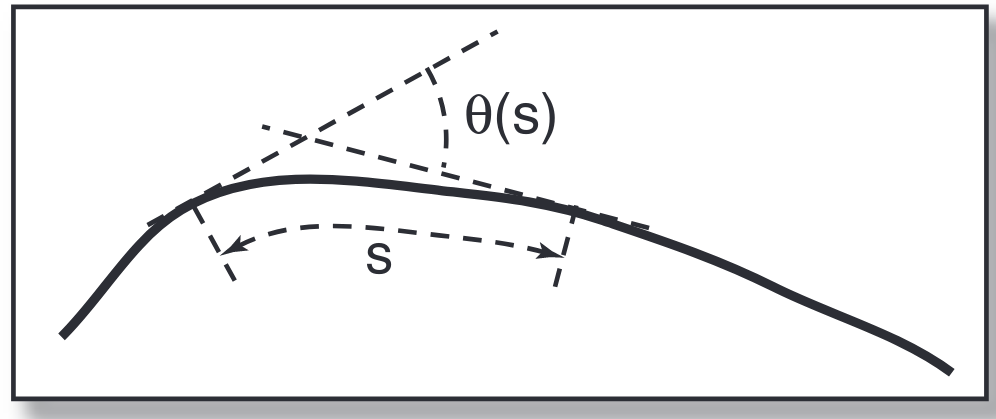
\includegraphics[width=75mm]{persistance_length.png} 
    \caption{Image taken from Grosberg \textit{et al.} 2011\cite{grosbergGiantMoleculesHere2011}. Angle formed between the tangents at the extremes of a contour length.} 
    \label{examplelabel} 
\end{figure}

The concept of persistance length is used in the polymer model to compute the angle bending potentials, which is calculated as in equation \ref{eq: angle bending potential}. For a DNA polymer, the Kuhn length is thought to be approximately equal to 100 nm. For this project, the relation between the persistance length and the latter was set to be as in equation \ref{eq: persistence length}.

% The Young's modulus ($E$) of a chain is the extent to which a solid material (or a polymeric fluid, in this case) can be deformed
% As Robert Hook noticed, the following is valid 
% \begin{equation}
    %     \sigma = E \frac{\Delta l}{l}
% \end{equation}
% Where $l$ represents the length of the chain and $\Delta l$ the deformation $\sigma$
% \cite{grosbergGiantMoleculesHere2011}

% The entanglement length ($N_e$) corresponds to the Young's modulus that is experimentally found in the plateau region where a force starts to produce irreversible deformations in a chain.

% % #TODO put a reference image if you want


% It is also defined as the "the average number of monomer units along the chain between two nearest effective cross-links."
% and is related to the ability of chains to form knots between each other
% \cite{grosbergGiantMoleculesHere2011}
.

%#TODO add subchapter rosettes
%#TODO about the reason of coarse graining with such a low resolution
%#TODO fine scale e coarse grained model, explain reasons
